\chapter[Throwing Polarised Light on some Mathematics]{Throwing Polarised Light on some Mathematics}\label{chap13}

\Authorline{Rajaram Nityananda\footnote[*]{Email: \url{rajaram.nityananda@gmail.com}}}

\authinfo{Senior Professor, Azim Premji University, Bengaluru}

The physics of a plane, perfectly monochromatic wave is simply summarised
in the electric field vector whose two orthogonal components are given by
$E_1 = a_1 \cos(wt - \phi_1)$; $E_2 = a_2 \cos(wt - \phi_2)$ or using basis vectors $\hat{e}_1$ and $\hat{e}_2$
\begin{gather*}
\overrightarrow{E} = Re (a_1 e^{i \phi_1 } \hat{e}_1 + a_2 e^{i\phi_2} \hat{e}_2 ) e^{-i\omega t} \\
\equiv Re \overrightarrow{\varepsilon} e^{-i\omega t}
\end{gather*}

The coefficient of the harmonic time dependence $e^{-i \omega t}$ is the complex two dimensional vector
$\overrightarrow{\varepsilon} = z_1 \hat{e}_1 + z_2 \hat{e}_2$ where $z_1$, $z_2$ encode the amplitude and the phase of each of
the components $- z_1 = a_1 e^{i \phi_1}$, $z_2 = a_2 e^{i\phi_2}$. Mathematician's call such a space
$\mathbb{C}^2$ (for two dimensional complex vector space). The operation which comes
naturally with such a space also have natural physical counterparts.
\begin{itemize}
\item[a)] Superposition $\overrightarrow{\varepsilon}_1 + \overrightarrow{\varepsilon}_2$ is realised as interference e.g using a half silvered
mirror as in the Michelson interferometer $\overrightarrow{\varepsilon}$ is proportional to $\overrightarrow{\varepsilon}_1 + \overrightarrow{\varepsilon}_2$ (ideally
$\frac{1}{\sqrt{2}} (\overrightarrow{\varepsilon}_1 + \overrightarrow{\varepsilon}_2)$)
\bigskip

\begin{figure}[H]
\centering
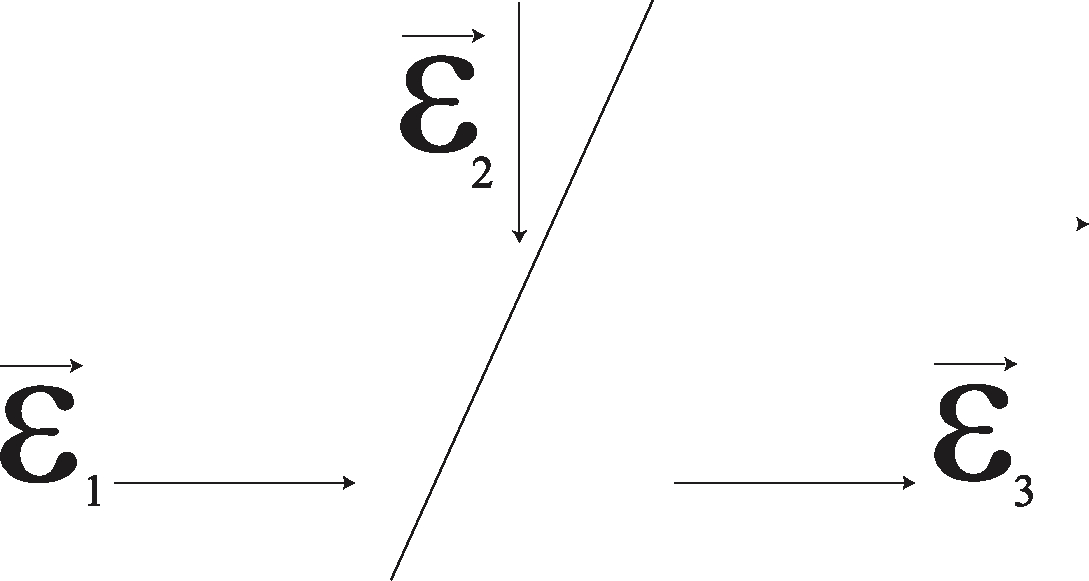
\includegraphics[scale=0.2]{src/images/chap26/1.jpg}
\end{figure}

\item[b)] Scalar multiplication $\overrightarrow{\varepsilon}' \to re^{i\theta} \overrightarrow{\varepsilon}$ for $r < 1$ this is the attenuator (dark
glass!) which cuts down the amplitude by $r$, $\theta$ is a phase retardation (parallel slab of transparent glass), $r > 1$, amplification also became possible after lasers


\item[c)] Norm in a complex vector space is the counterpart of ``squared length" in
our familiar vectors. The intensity of our wave is proportional to $a_1^2 + a_2^2$ after
averaging over a period. This can be written as $I = | z_1 |^2 + | z_2 |^2$ $\equiv z^{\ast}_1 z_1 + z^{\ast}_2 z_2$ $\equiv \overrightarrow{\varepsilon}^{\ast} \cdot \overrightarrow{\varepsilon}$ (notice that $\ast$ in over the first $\overrightarrow{\varepsilon}$, it's important)

\item[d)] A typical experiment is to combine two different beams $\overrightarrow{\varepsilon}$ and $\overrightarrow{\varepsilon}'$ apply a phase
shift $\psi$ to $\overrightarrow{\varepsilon}'$, and measure the total intensity, using (a), (b) and (c) above, this
gives:
\begin{align*}
I_{tot} & = (\overrightarrow{\varepsilon}^{\ast} + \overrightarrow{\varepsilon}'^{\ast} e^{-i\psi})  \cdot (\overrightarrow{\varepsilon} + \overrightarrow{\varepsilon}' e^{i\psi})\\
& = \overrightarrow{\varepsilon}^{\ast} \cdot \overrightarrow{\varepsilon} + \overrightarrow{\varepsilon}'^{\ast}  \cdot \overrightarrow{\varepsilon}' + (\overrightarrow{\varepsilon}^{\ast} \cdot \overrightarrow{\varepsilon}' e^{i\psi}  + \text{ its complex conjugate}).
\end{align*}
The first two terms are just the intensity of $\overrightarrow{\varepsilon}$ and $\overrightarrow{\varepsilon}'$ by themselves. Our focus will be on the interference term which can be written out in full as $Re(\overrightarrow{\varepsilon}^{\ast}  \cdot \overrightarrow{\varepsilon}') \cos \psi + \Iim (\overrightarrow{\varepsilon}^{\ast} \cdot \overrightarrow{\varepsilon}') \sin \psi$
Since $\psi$ can be varied, both the real and imaginary parts of ($\overrightarrow{\varepsilon}^{\ast} \cdot \overrightarrow{\varepsilon}'$) can be
measured. Mathematically, this is the ``inner product", and the norm is just
the inner product of a vector with itself. We can also write the interference
term as $\| \overrightarrow{\varepsilon}^{\ast}  \cdot \overrightarrow{\varepsilon}'\| e^{i\phi_{EE'}} \cdot e^{i\psi}$ where $\phi_{\varepsilon \varepsilon'}$ is the phase of our inner product and $\psi$ our added phase in the $\varepsilon'$ beam. The intensity of this term now reads
$| \overrightarrow{\varepsilon}^{\ast} \cdot \overrightarrow{\varepsilon}| \cos (\phi_{EE'} + \psi)$ and is a maximum when $\psi = -\phi_{EE]}$. Pancharatnam
used this criterion to define the phase retardation of $\overrightarrow{\varepsilon}'$ with respect to $\varepsilon$, when
they are in different states of polarization. Namely, since retardation of $-\phi_{\varepsilon \varepsilon}'$ 
given to $\varepsilon'$ maximises the intensity, i.e, brings them `in phase', it's logical to
think of $\phi_{\varepsilon \varepsilon'}$ in this way. We will return to this later!

\item[e)] The definition fails in one case, when the inner product is zero. The simplest
example would be $\varepsilon = \alpha \hat{e}_1$, $\varepsilon = \alpha' \hat{e}_2$. This is one of the ``Fresnel Argo laws" for
interference of polarized light - two linearly polarized beams in perpendicular
directions do not interfere. More correctly, we should say that as we vary the
relative phase, the intensity does not change. We can see that any two beams
satisfying $a^{\ast} \cdot b = 0$ will show this non interference in intensity - they are called
orthogonal.

\item[f)] So far, our vectors have been expressed in terms of $\hat{e}_1$ and $\hat{e}_2$, two unit intensity
linearly polarized beams. A vector space like $\mathbb{C}^2$ comes with the freedom to
change the basis. For example, define $\hat{e}_R = \frac{\hat{e}_1 + i \hat{e}_2}{\sqrt{2}} ~~\&~~ \hat{e}_L = \frac{\hat{e}_1 - i \hat{e}_2}{\sqrt{2}}$. It is easily
checked that $\hat{e}^{\ast}_R  \cdot \hat{e}_R = \hat{e}^{\ast} \cdot \hat{e}_L = 1$ and $\hat{e}^{\ast}_R \cdot \hat{e}_L = 0$. Any vector can be rewritten
in terms of $\hat{e}_R$ and $\hat{e}_L$ as follows - easily verified.
\end{itemize}
$\overrightarrow{\varepsilon} \equiv Z_1 + \hat{e}_1 + Z_2 \hat{e}_2  \equiv Z_R \hat{e}_R + Z_L \hat{e}_L$ where the amplitudes of the $R$ and $L$ beams are 
$$
Z_R  = \dfrac{Z_1 + iZ_2}{\sqrt{2}} ; ~~ Z_L = \dfrac{Z_1 - iZ_2}{\sqrt{2}}
$$
$\hat{e}_R$ and $\hat{e}_L$ are just one example of an orthonormal basis pair but have a simple
physical meaning. $\hat{e}_R$ is an equal superposition of beams along $x$ and $y$, with
$y$ retarded by a phase lag of $\pi/2$ (hence the i in front of $\hat{e}_2$). In such a beam,
the tip of the electric vector describes a circle, ($E_x = a \cos wt$, $E_y = a \sin wt$)
traversed counter clockwise when facing the source. This is called `right circularly polarized' or RCP light. Retarding it in phase moves the vector clockwise.
LCP has the the opposite sense since $E_y$ leads $E_x$ by $\pi/2$. RCP carries angular
momentum along the direction of propagation and LCP opposite to it (like off
spin and leg spin in cricket!)
\smallskip

\begin{figure}[H]
\centering
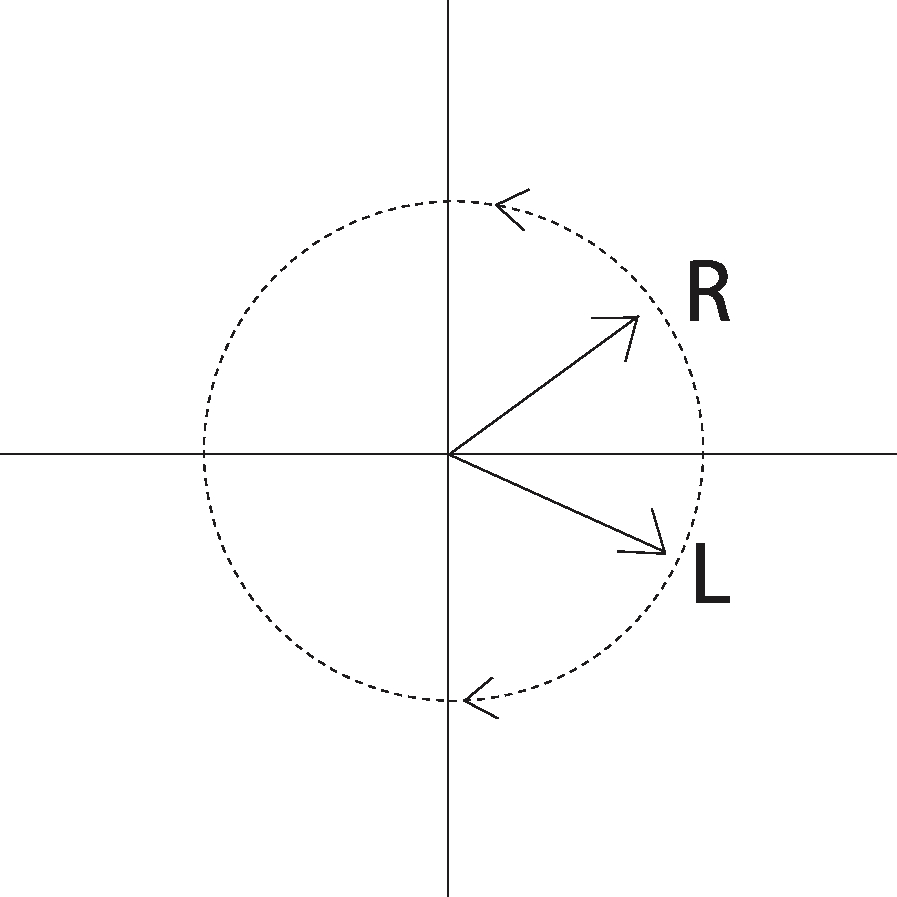
\includegraphics[scale=0.25]{src/images/chap26/2.jpg}
\end{figure}
\bigskip

The two complex amplitudes $z_R$ and $z_L$ are very convenient to understand
the result of general superposition, geometrically. Assuming $| z_R |>| z_L |$ and
their phases to be $\phi_R$ and $\phi_L$. The situation at $t = 0$ is as in the figure. (where $\phi_R$ and $\phi_L$ are taken $> 0$)
\medskip

\begin{figure}[H]
\centering
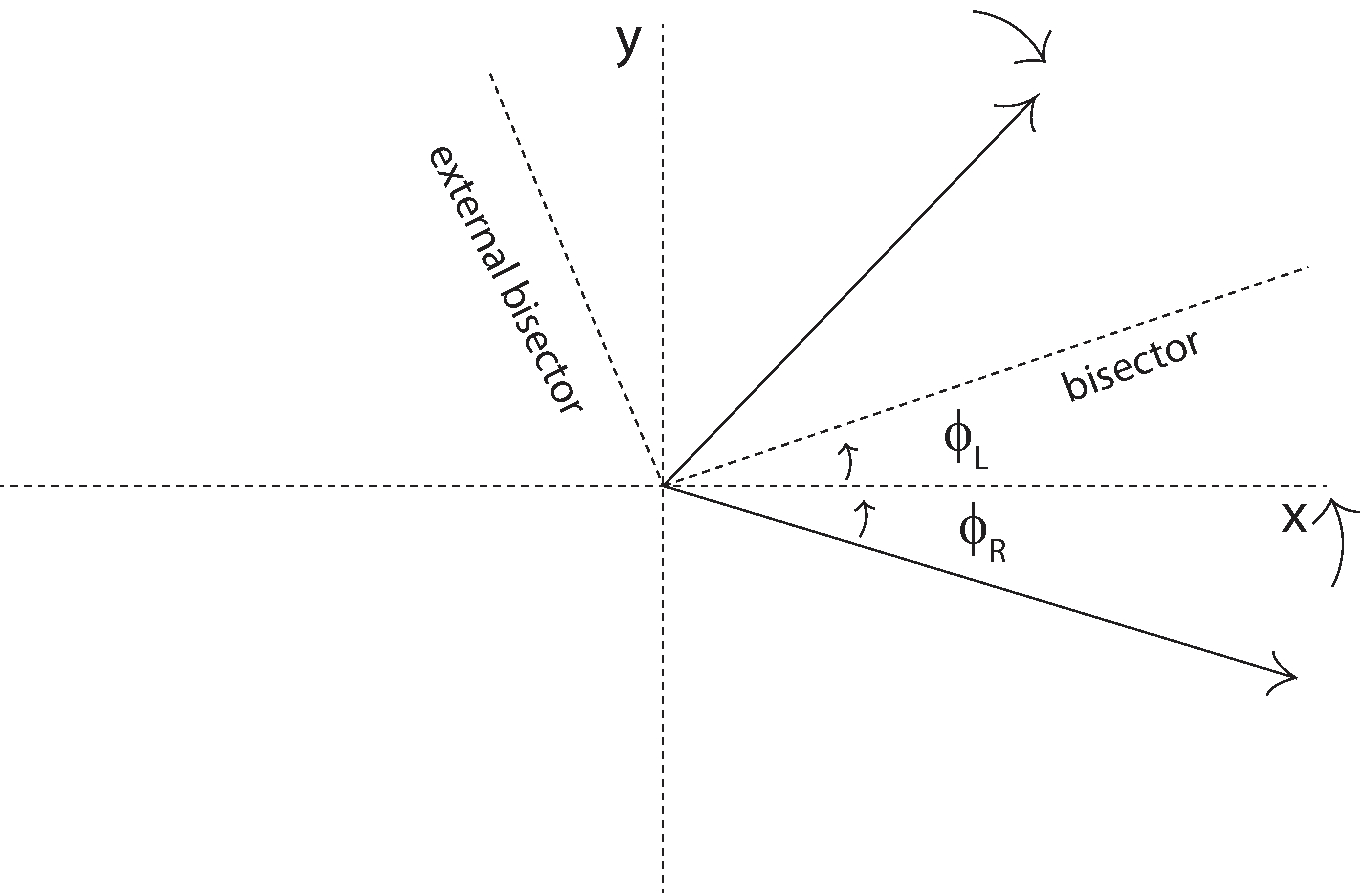
\includegraphics[scale=0.25]{src/images/chap26/3.jpg}
\end{figure}
\bigskip

Clearly, the two vectors will become parallel on the bisector at $\alpha = (\phi_L -\phi_R)/2$ 
with respect to $x$ axis and the electric field will attain its maximum value
$| z_R | + | z_L |$.

Quarter of a period later $| z_L |$ will point oppositely to $| z_R |$ and the field
will take its minimum value of $| z_R | - | z_L |$. The resulting path or orbit of the
tip of the electric vector is thus an ellipse and the ratio of axis is $\frac{|z_R| - |z_L|}{|z_R| + |z_L|} = \frac{1-|\frac{z_L}{z_R}|}{1+|\frac{z_L}{z_R}|}$
with major axis along $\frac{\phi_L -\phi_R}{2}$. This is called elliptically polarized light
and with $|z_R | > |z_L |$, the the ellipse is traversed counterclockwise, hence right
handed. If $|z_R | < |z_L |$, our formula for axial ratio goes negative and the ellipse
is now left rotating. Clearly right circular light $\Rightarrow |\frac{Z_L}{Z_R}| = 0$ and left circular $|\frac{Z_R}{Z_L}| =0$ or $\frac{Z_L}{Z_R} \to \infty$. 
 Notice that our formula for the direction of major axis is
ambiguous - if we change $\phi_L$ or $\phi_R$ by a multiple of $2\pi$, the `azimuth' $\alpha$ changes
by a multiple of $\pi$. This is actually desirable, because the major axis has two
ends whose azimuth differs by $\pi$. Thus we write $\phi_L - \phi_R = 2\alpha$ and now both
sides are ambiguous to $2n\pi$ which all angles should be anyway. Thus the shape
and orientation of the polarization ellipse is contained in the magnitude $\left(\frac{Z_R}{Z_L} \right)$
and phase $(\phi_L - \phi_R$) of the single complex number $\zeta = \frac{Z_L}{Z_R}$. This is, again, a
mathematical idea, now one which is not taught in physics courses even at the
masters level.


From $\mathbb{C}^2$ which is made up of pairs ($z_L , z_R$) we have retained only the relative
amplitude and phase difference, by forming $\zeta = \frac{z_L}{z_R}$. Further, as $z_R \to 0$, $\zeta$
goes to $\infty$ in a direction set by the phase of $Z_R$. But $Z_R = 0$ is a unique point,
as far as polarization is concerned viz LCP. The mathematicians also felt the
need for a single point at infinity in the complex plane of $\zeta$ and achieved it by
``Riemann sphere" using  ``stereographic projection" - both terms are explained
better by a figure.
\medskip

\begin{figure}[H]
\centering
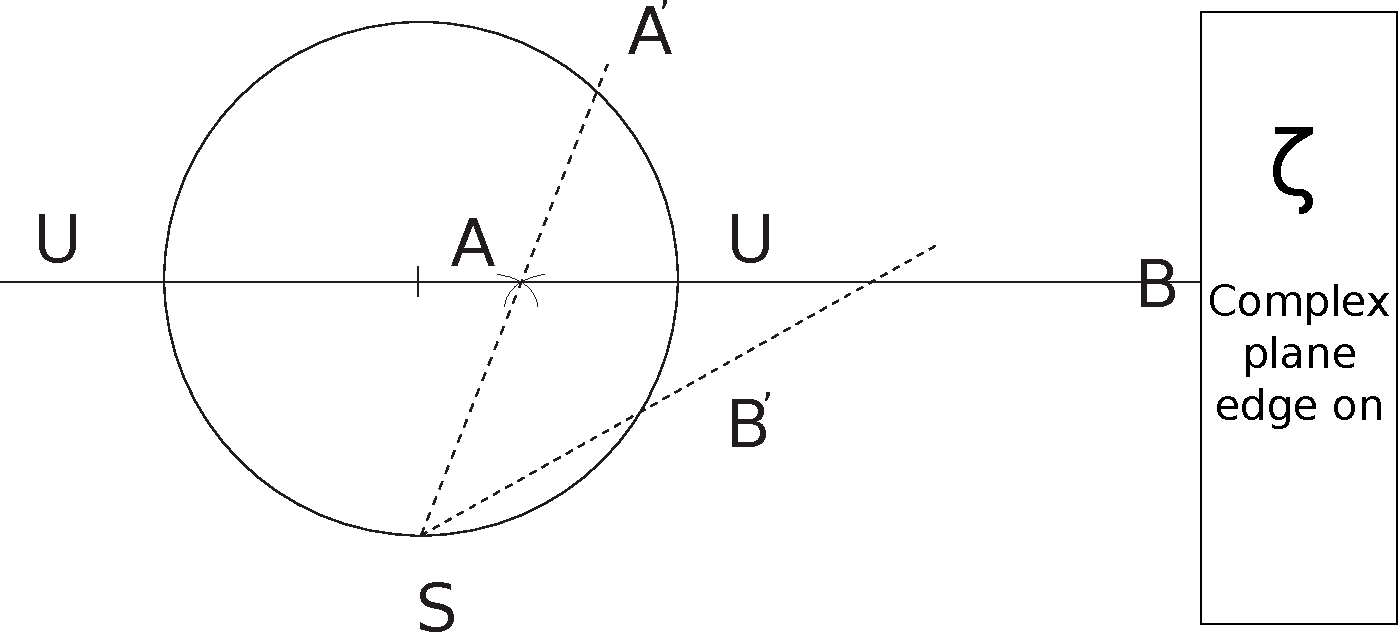
\includegraphics[scale=0.2]{src/images/chap26/4.jpg}
\end{figure}
\bigskip

A B are mapped onto $A'$, $B'$ on the sphere by projection from $S$. The sphere
has unit radius and $U U$ is a unit circle.


The geometry of the projection brings out the connection between the polar
angles $\theta$, $\phi$ on the Riemann sphere and the complex number, viz, $\zeta = \tan \frac{\theta}{2} e^{i\phi}$.
\medskip

\begin{figure}[H]
\centering
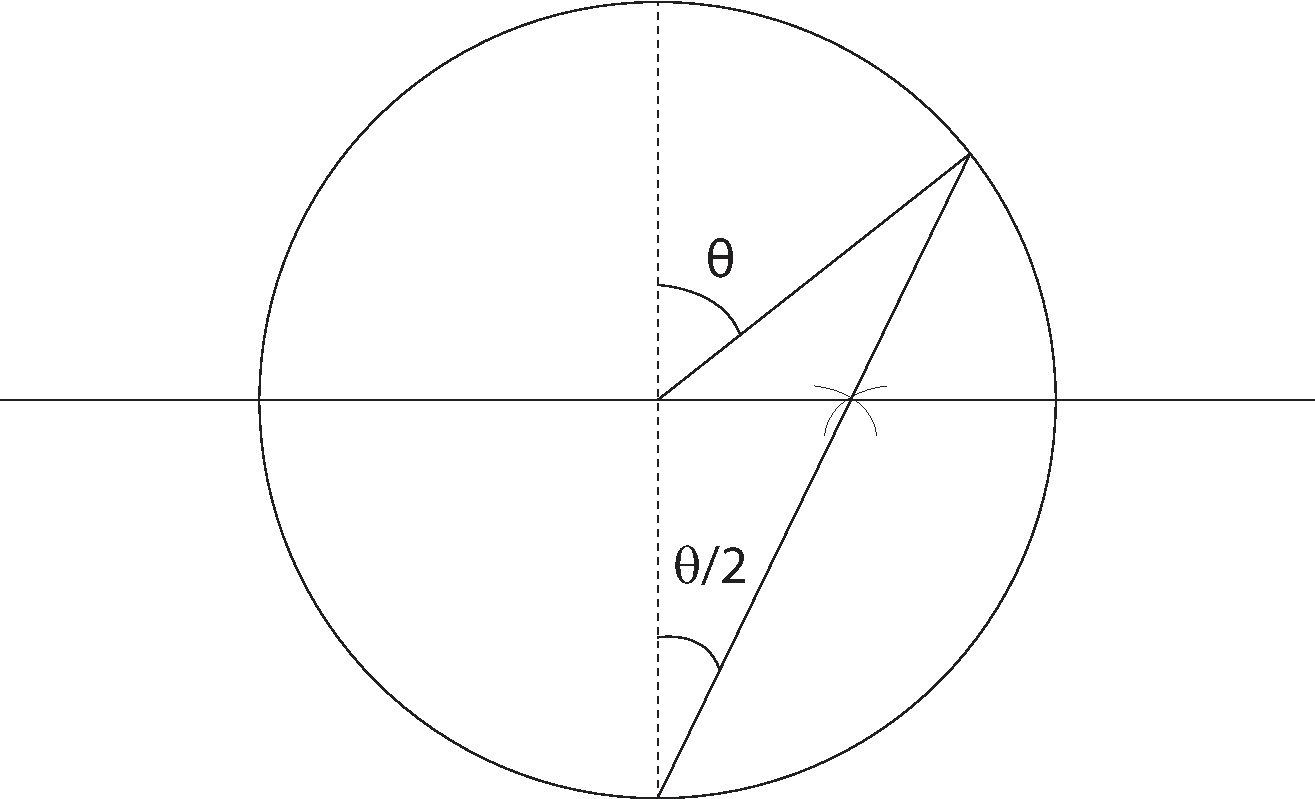
\includegraphics[scale=0.2]{src/images/chap26/5.jpg}
\end{figure}
\bigskip

Mathematically, we have gone from $\mathbb{C}^2$, where a point is ($z_R , z_L$) to a ``complex projective space with one dimension" known a $\mathbb{C}P^1$. We can think of it
as the space of $\zeta$ but including the point at infinity, so its better to think of it
as Riemann sphere. We are concentrating on the shape of the ellipse and
igoring its size (by taking the axial ratio), and also ignoring phase (by looking
at the whole orbit and not just one point on it). We are really saying that two
points on $\mathbb{C}^2$, viz ($z_R , z_L$) and ($\lambda z_R , \lambda z_L$) with $\lambda = re^{i\theta}$, $r\neq 0$, are the same
point in $\mathbb{C}P^1$ - the projection is really this equivalence relation. The result is to
map all ellipses onto a sphere, which was invented by Poincare'. (19 and early
$20^{\rm th}$ century French mathematician ). The dictionary goes as follows -right circular on the north pole, LCP at the south pole, and at $\theta$ not equal to zero or
$\pi$, the axial ratio of the ellipse is
\begin{align*}
\frac{1-\tan \theta /2}{1+ \tan \theta /2} & \equiv \frac{\cos \frac{\theta}{2} \cos \frac{\pi}{4} - \sin \frac{\theta}{2} \sin \frac{\pi}{4}}{\cos \frac{\theta}{2} \cos \frac{\pi}{4} + \sin \frac{\theta}{2} \sin \frac{\pi}{4}}\\
& = \frac{\cos (\frac{\pi}{4} + \frac{\theta}{2})}{\cos (\frac{\pi}{4} - \frac{\theta}{2})} = \frac{\sin (\frac{\pi}{4} -\frac{\theta}{2})}{\cos (\frac{\pi}{4} - \frac{\theta }{2})}\\
& = \tan \frac{(\frac{\pi}{2} -\theta)}{2} = \tan \left(\frac{latitude}{2} \right)
\end{align*}

The equator, latitude $= 0$, corresponds to linearly polarized light. Indeed,
it is an important idea of elementary optics that a linear beam can be thought
of as superposition of two circular beams, with opposite senses. As we vary the
phase difference between them, the azimuth of the linear beam changes by half
that phase change. This is what happens in sugar solution and quartz crystals,
telling us that these come in two different mirror image forms which rotate the
direction of linear polarization in opposite ways. More fundamentally, even an
atom like Cs has shown this effect, though minutely - evidence for the violation
of mirror symmetry in the the basic electromagnetic interaction, because of its
unification with the weak interaction. A `map' of the poincare sphere, similar
to the world map in the atlases, would look like this.
\bigskip

\begin{figure}[H]
\centering
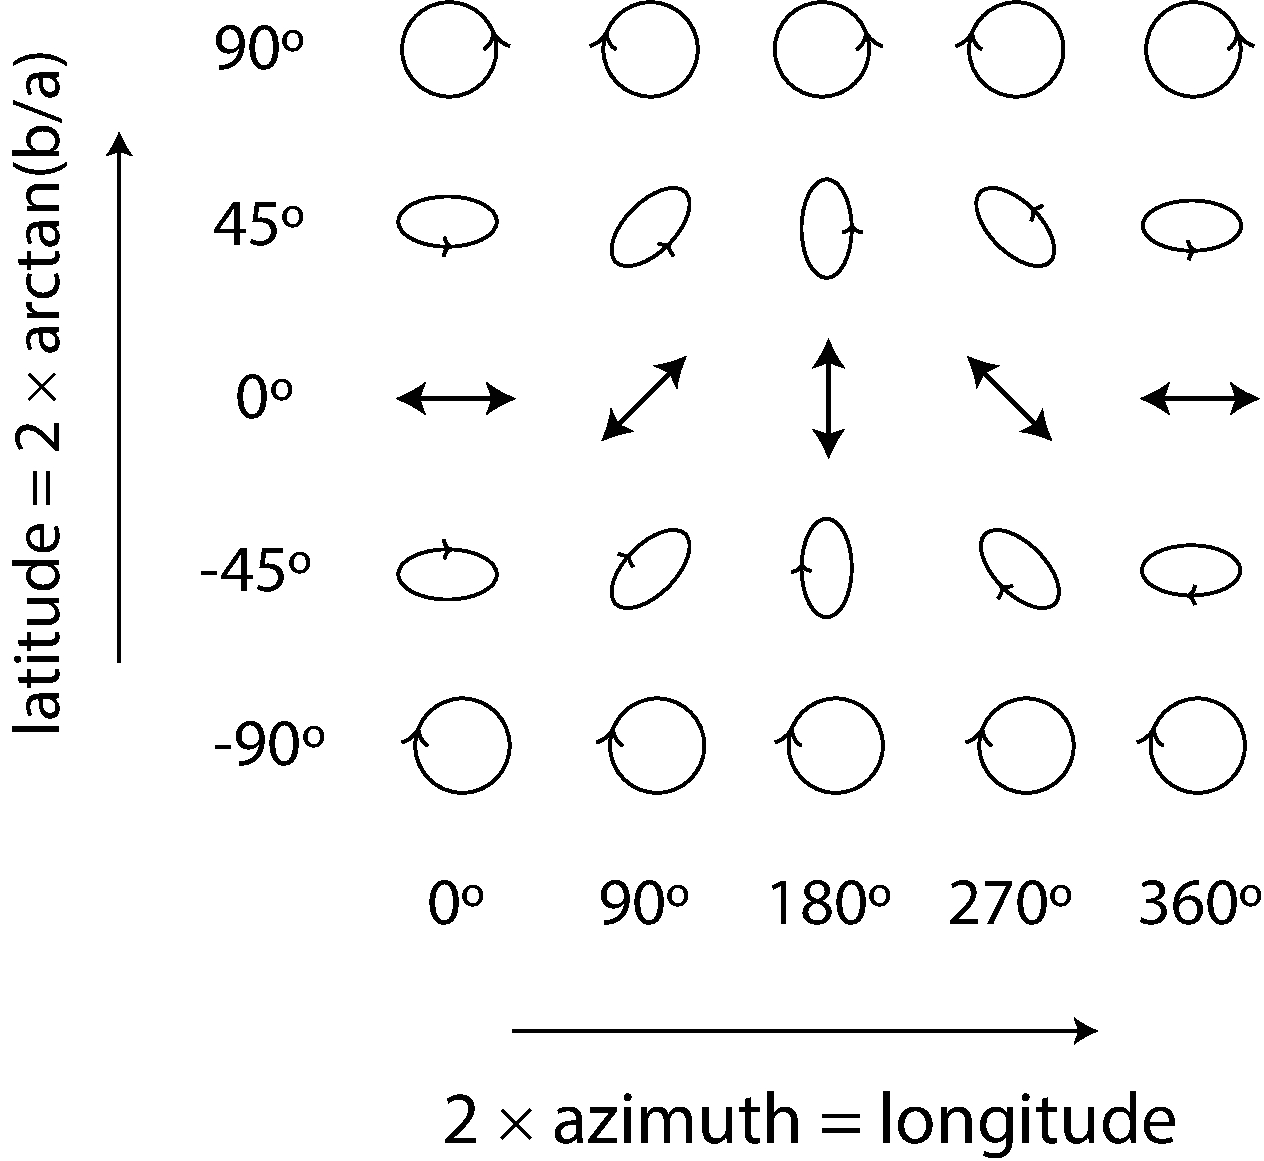
\includegraphics[scale=0.21]{src/images/chap26/6.jpg}
\end{figure}

Like the world map, this represents a sphere as a rectangle, with understand-
ing that the left and right edges are the same. Also, the north and south poles
are not lines but points, because latitude is irrelevant (what is the major axis of
a circle?). This map should convince even a lay person that the sphere is the
correct topology for the space of all states (orbits) of polarised light. Indeed,
Poincare’ was a pioneer of topology, but his sphere achieved more as we will
see. One clue is that our two examples of orthogonal states, viz. horizontal and
vertical, as well as LCP and RCP, lie at opposite - antipodal - points on the
sphere. This is a particular case of a general result whose proof is given below
- magnitude of interference term, or inner product, between any two points on
the Poincare' sphere, is given by $\cos(\gamma/2)$ where $\gamma$ is the angle subtended at the
centre by these two points. The calculation assumes that the two fields $\overrightarrow{\varepsilon}$ and
$\overrightarrow{\varepsilon}'$ are normalised, hence
\begin{align*}
\overrightarrow{\varepsilon} & = \cos \frac{\theta}{2} e^{i \xi_1} \hat{e}_R + \sin \frac{\theta}{2} e^{i(\xi_1+ \phi)} \hat{e}_L\\
\overrightarrow{\varepsilon}' & = \cos \frac{\theta'}{2} e^{i \xi'_1} \hat{e}_R + \sin \frac{\theta'}{2} e^{i (\xi'_1 + \phi')} \hat{e}_L
\end{align*}

In writing this form, the ratio $Z_L /Z_R = \tan \theta/2$ and phase difference $\phi$ have
been incorporated apart from the unit intensity.
\bigskip

\begin{figure}[H]
\centering
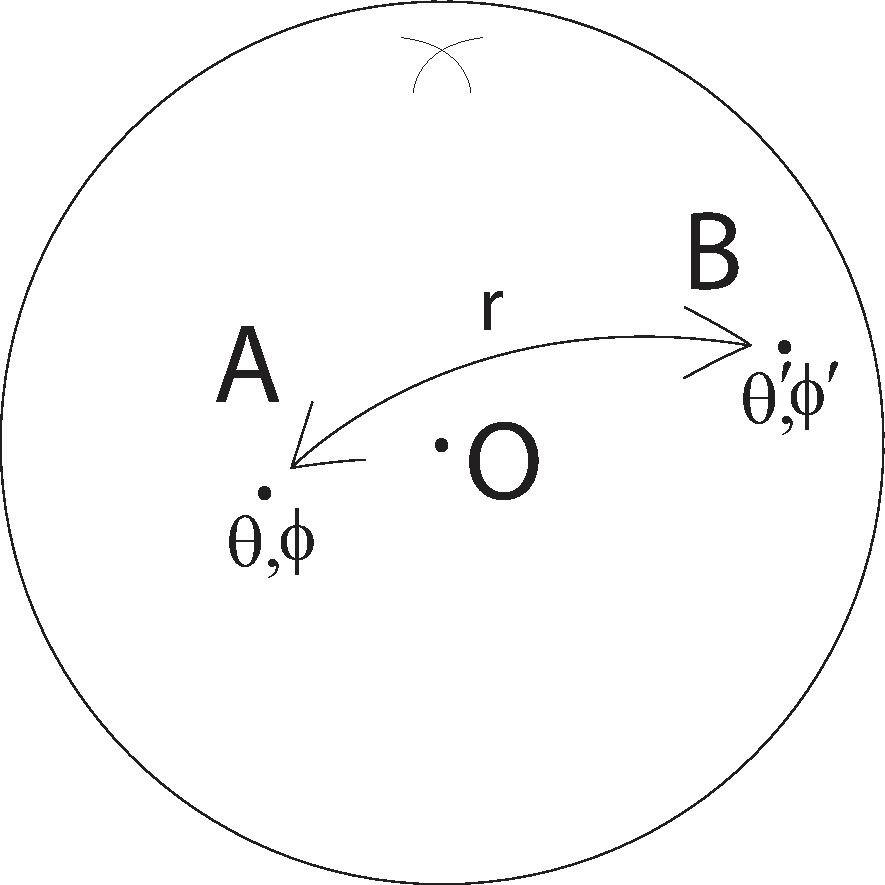
\includegraphics[scale=0.21]{src/images/chap26/7.jpg}
\end{figure}
\bigskip

Writing out $\overrightarrow{\varepsilon} \ast \cdot  \overrightarrow{\varepsilon}'$ in full, we have
$$
\overrightarrow{\varepsilon} \ast \cdot \overrightarrow{\varepsilon}' = \cos  \frac{\theta}{2} \cos \frac{\theta'}{2} e^{i (\xi'_1 - \xi_1)} + \sin \frac{\theta}{2} \sin \frac{\theta'}{2} e^{i (\xi'_1 - \xi_1)} e^{i \phi'}
$$

Note that if we are only interested in the magnitude of the inner product, the
common factor $e^{i(\xi_1 - \xi'_1)}$ can be removed - how could it be otherwise. Since the
Poincare' sphere doesn't represent phase of a beam (or its intensity). We now
square and add the real and imaginary parts to get the square of our desired
magnitude viz
$$
\left(\cos \frac{\theta'}{2} \cos \frac{\theta}{2} + \sin \frac{\theta}{2} \sin \frac{\theta'}{2} \cos (\phi - \phi') \right)^2 + \left(\sin \frac{\theta}{2} \sin \frac{\theta'}{2}
\sin \phi\right)^2
$$

It is a nice exercise in trigonometry to get this to the form $\frac{1}{2} [1 + \cos \theta . \cos \theta' +
\sin \theta \sin \theta'  \times \cos (\phi - \phi')]$ and inside the brackets, apart from 1, is the ordinary real dot product of the
vectors OA and OB. Hence we have
$$
|\text{inner product}|^2 = \frac{1}{2} (1 + \cos \gamma) = \cos^2 (\gamma/2) \qquad {Q.E.D}
$$


As a byproduct, two orthogonal states always lie at the antipodes of each
other. i.e. $\theta$, $\phi$ and $\pi - \theta$, $\phi + \theta$. We can see that the two points lie at the
same latitude but one S and one N, hence same axial ratio, oppositely traversed.
The $\pi$ difference of longitudes translates to $\pi/2$ in azimuth, hence the general
orthogonal pair looks like
\medskip

\begin{figure}[H]
\centering
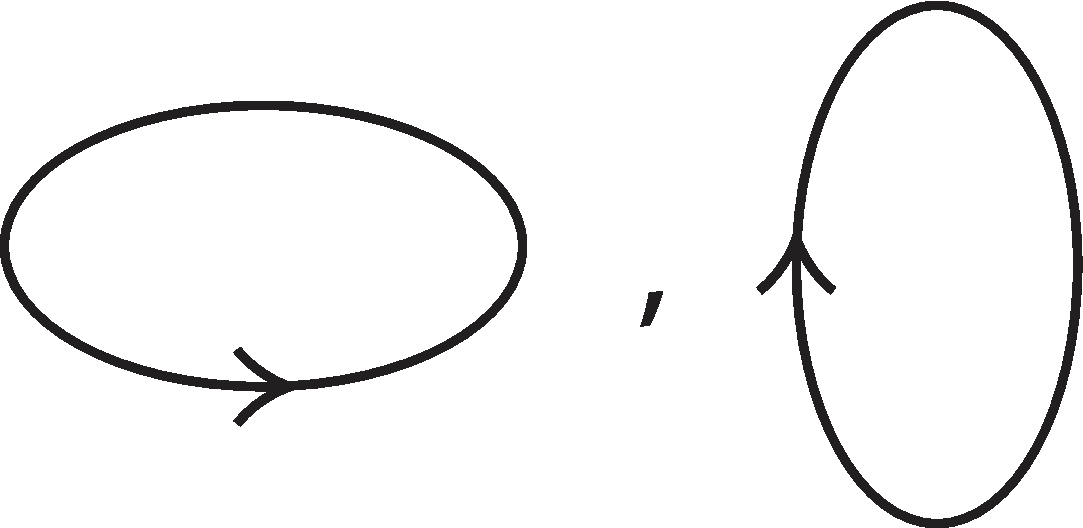
\includegraphics[scale=0.25]{src/images/chap26/8.jpg}
\end{figure}
\bigskip

It's also easy to check, in our old $e_1$, $e_2$ basis that the dot product of ($\hat{e}_1 + i (\frac{b}{a}) \hat{e}_2)^{\ast}$ and ($\hat{e}_2 + i(\frac{b}{a}) \hat{e}_1)$ is zero.

The Poincare' sphere has many nice properties. We have seen how an equal
combination of two orthogonal (L and R) states with varying phase difference
moved the resulting linear state around the equator. The same holds for any
two orthogonal states, viz H and V can again combine to give linear, elliptic,
circular as one traverses an arc of longitude.
\bigskip

\begin{figure}[H]
\centering
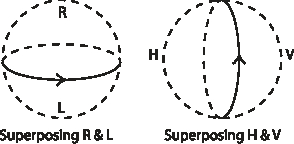
\includegraphics[scale=1.2]{src/images/chap26/9.jpg}
\end{figure}
\bigskip

This is a good way to understand quarter wave plates, half wave plates,
etc - for those with geometric bent, (there are Jones and Muller matrices for
those who prefer the left hemisphere). These generalize to unequal superpositions,
and non-orthogonal states - a good reference, not easy to get nowadays, is a
\textit{Handbook der Physik} article by \textit{Ramachandran and Ramaseshan}. But we set
these aside, to treat the central topic of these lectures, the Pancharatnam(P)
phase. We have already mentioned his physically motivated definition of the
phase difference between two beams, viz the phase of the inner product $\overrightarrow{\varepsilon}^{\ast} \cdot \overrightarrow{\varepsilon}'$. 
Motivated by his own experiments on the interference of polarised light in absorbing bifrigent crystals - which we will only touch upon, later - he asked and
answered the following fundamental question. Again, using mathematical language that Pancharatnam did not, is the relation of two differently polarized
$\overrightarrow{\varepsilon}$ and $\overrightarrow{\varepsilon}'$ being `in phase' an `equivalence relation'? i.e. is $\varepsilon$ in phase
with $\varepsilon$? - yes since the phase of $\overrightarrow{\varepsilon}^{\ast} \cdot \overrightarrow{\varepsilon}$ is zero. 
If $\overrightarrow{\varepsilon}$ is in phase with $\overrightarrow{\varepsilon}'$, 
i.e.\ $\overrightarrow{\varepsilon}^{\ast} \cdot \overrightarrow{\varepsilon}'$ is real, 
then so is $\overrightarrow{\varepsilon}'^{\ast} \cdot \overrightarrow{\varepsilon}$; 
and hence $\overrightarrow{\varepsilon}'$ is in phase with $\overrightarrow{\varepsilon}$. 
But now comes the `punch' line. Let us say $\overrightarrow{\varepsilon}$ is in phase 
with $\overrightarrow{\varepsilon}'$ and $\overrightarrow{\varepsilon}'$ is in phase with $\overrightarrow{\varepsilon}''$. 
A lesser man would have concluded that $\overrightarrow{\varepsilon}''$ is in phase with $\overrightarrow{\varepsilon}$, 
but no, it is not, the difference is the P phase, a property of the triplet 
$\overrightarrow{\varepsilon}$, $\overrightarrow{\varepsilon}'$, $\overrightarrow{\varepsilon}''$, which he 
was able to calculate, with subtle physical and geometric arguments, and express in
terms of the location on the Poincare sphere in a most beautiful form - it is half
the solid angle made at the centre of the sphere by the three points representing
$\overrightarrow{\varepsilon}$, $\overrightarrow{\varepsilon}'$, $\overrightarrow{\varepsilon}''$. We start with an example - three states which are on the Poincare sphere.
\bigskip

\begin{figure}[H]
\centering
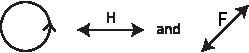
\includegraphics[scale=0.85]{src/images/chap26/10.jpg}
\end{figure}
F stands for forty five.

The three electric fields are
\bigskip

\begin{figure}[H]
\centering
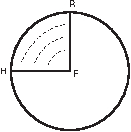
\includegraphics[scale=1]{src/images/chap26/11.jpg}
\end{figure}
$$
\overrightarrow{\varepsilon}_R = \left(\frac{\hat{e}_1 + i \hat{e}_2}{\sqrt{2}} \right); ~ \overrightarrow{\varepsilon}_H = \hat{e}_1 ; ~~ \overrightarrow{\varepsilon}_F = \frac{\hat{e}_1  + \hat{e}_2}{\sqrt{2}}
$$

And the phases of the three inner products are easily seen to be $\phi_{RH} = 0$; $\phi_{HF} =0$, and $\phi_{FR} =$ phase of $\frac{(1+i)}{2} = \pi/4$, which is exactly half of $\pi/2$ (one eighth of the full sphere of $4\pi$) which agrees with the general result. One comment - this is not a consequence of the specific overall phases we chose for R, H, F - in fact, more generally, the triple product $(\overrightarrow{\varepsilon}^{\ast} \cdot \overrightarrow{\varepsilon}')(\overrightarrow{\varepsilon}'^{\ast} \cdot \overrightarrow{\varepsilon}'')(\overrightarrow{\varepsilon}''^{\ast} \cdot \overrightarrow{\varepsilon})$ is invariant if we change the phase of any or all of the three beams, because each occurs once with a star and once without. This observation predates P - \textit{Bargmann} made and used it in a more mathematical context. The invariance
to phases allows us to calculate it on the Poincare sphere.

In a short set of lectures - and notes - we will not take P’s route to the half
solid angle formula. But those with taste of geometry could go to the original
papers - I wrote a piece in current science; Aug 1994 on \textit{`Pancharatam's route
to the geometry phase'} (accessible by typing the title in a google window )
which sketches the derivation and may be helpful. We will reach it from a
more analytical viewpoint, by calculating the phase going around a quadrilateral
$ABCD$, with
\smallskip

\begin{figure}[H]
\centering
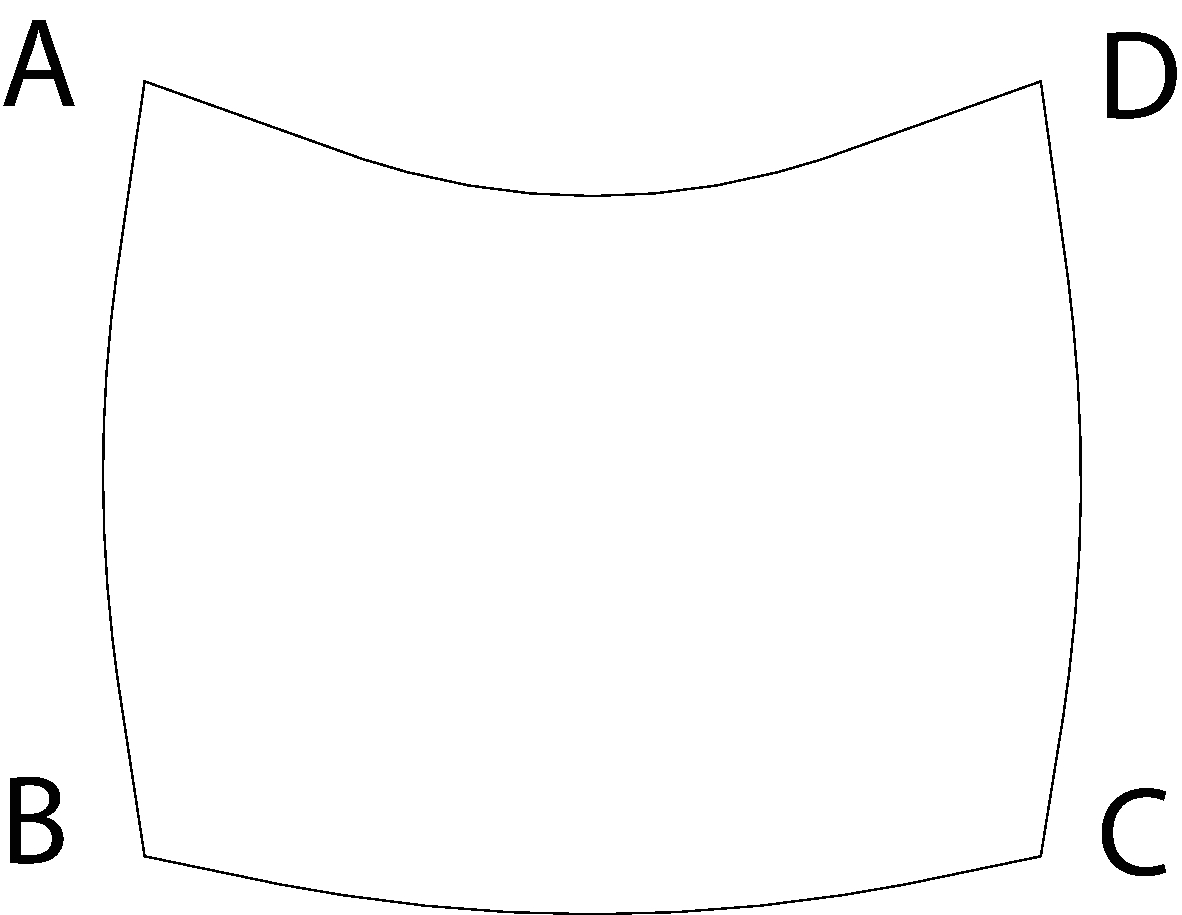
\includegraphics[scale=0.16]{src/images/chap26/12.jpg}
\end{figure}
\begin{gather*}
A = (\theta, \phi),\\
B = (\theta + \Delta \theta, \phi),\\
C = (\theta + \Delta \theta, \phi + \Delta \phi),\\
D = (\theta, \phi + \Delta \phi)
\end{gather*}

Using our standard form $(Z_R , Z_L ) = (\cos \frac{\theta}{2}, ~ \sin \frac{\theta}{2} e^{i\phi})$ we find the phases
of the four inner products to be
\begin{gather*}
\phi_{AB} = 0,\\
\phi_{BC} = \sin^2 \frac{(\theta + \Delta \theta)}{2} \cdot \Delta \phi,\\
\phi_{CD} = 0,
\end{gather*}
$phi_{DA} = -\sin^2 \frac{\theta}{2} \Delta \phi$, working to the lowest order in $\Delta \phi$. 
Now keeping only order $\Delta \theta$ as well, we get :
\begin{align*}
\phi_{ABCD} &= 2 \sin \frac{\theta}{2} \cos \frac{\theta}{2} \frac{\Delta \theta }{2} \Delta \phi\\
&= \frac{1}{2} \sin \theta \Delta \theta \Delta \phi.
\end{align*}

This is the standard expression for the solid angle enclosed by\break $ABCD$, apart
from the $\frac{1}{2}$. The value for a large circuit can be built up from this by addition -
the phase on common legs cancels. e.g.
\bigskip

\begin{figure}[H]
\centering
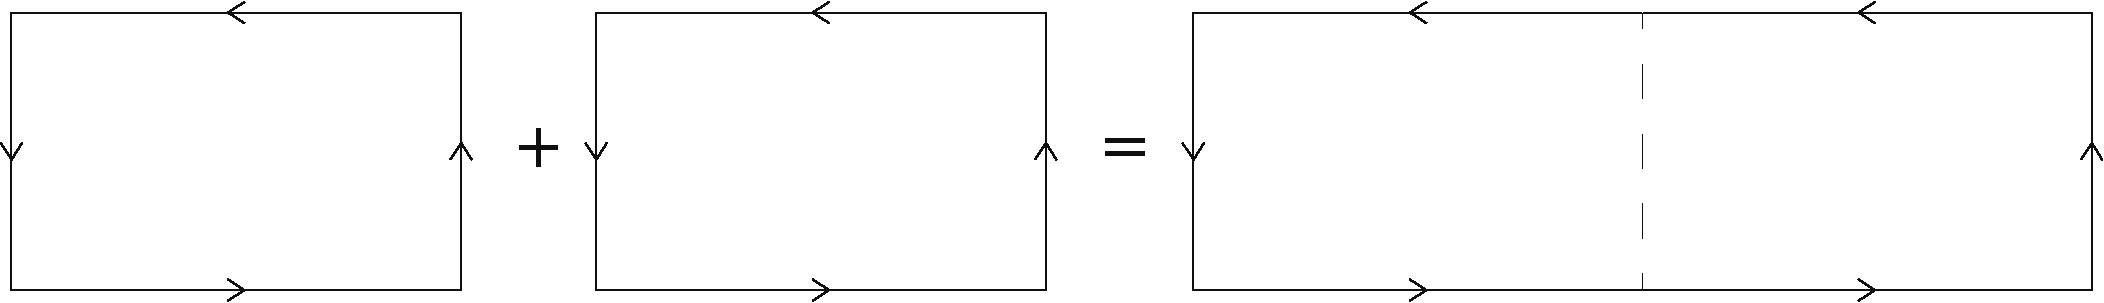
\includegraphics[scale=0.18]{src/images/chap26/13.jpg}
\end{figure}
\bigskip

Notice that if any two of the beams are in orthogonal polarisation states, the
corresponding inner product vanishes and the phase is undefined. It so happens
that in an absorbing crystal, iolite, the two modes are not orthogonal and when
they are combined and viewed through an analyser, say a polaroid, the proper
treatment of this experimental situation raised, atlest to a mind of sufficient
quality, the general question we have discussed, with hindsight.

These matters rested from 1955 to 1984 when \textit{Berry} introduced his rightly
famous phase for a quantum system R evolving adaibatically. His result was that
once the `dynamical phase' $\exp(-  \frac{i}{\not{h}} \int E ~dt)$  with slowly varying $E$ was removed,
the wave function, in this adiabatic limit, evolved so that $\psi(t + dt)$ was in phase
with $\psi(t)$ i.e, the inner product was real. Which meant, as we have seen, that
the phase around a closed circuit would be nonzero. Although we have been
talking about classical light beams, the basic tool has been a cmplex vector
space no different from that used in quantum mechanics. This `Berry phase'
(which he calls `geometric phase') is now a standard part in QM courses and a
subject in its own right. A later atricle by \textit{Berry} in \textit{Physics Today} documents
three or four earlier pieces of work which could be called anticipations of the
geometric phase and the \textit{Pancharatam} phase is one of them. We will now use
it to illustrate another mathematical concept, developed by \textit{Clifford} in the late
19$^{\rm th}$ century and by $Hopf$ in 1930's - Recall that we started with $\mathbb{C}^2$ made up
of pairs ($z_R, z_L$). Unit intensity would then lead to $| z_R |^2 + | z_L |^2 = 1$ which
is satisfied if we set $z_R = \cos \frac{\theta}{2} e^{i \xi_1}$ and $z_L = \sin \frac{\theta}{2} e^{i \xi_2}$. We now have three
parameters, $\theta$, $\xi_1$, $\xi_2$ and we singled out $\xi_2 - \xi_1$, as the phase difference $\phi$ (twice
the azimuth of the ellipse) leaving $\xi_1$ itself as an overall phase. What happens if
we put back $\xi_1$, i.e, restore the overall phase to the Poincare sphere? The unit
intensity condition, written in terms of real and imaginary parts of $z_R$ and $z_L$
$(z_R = x_R + iy_R, ~z_L = x_L + iy_L$) reads $x^2_R + y^2_R + x^2_L + y^2_L = 1$. This is the set of
points in $4-d$ space. $\mathbb{R}^4$, at a unit distance from the origin and is hence called the
3-sphere, $S^3$, just as $x^2 + y^2 = 1$, the circle, is $S^1$, and $x^2 + y^2 + z^2 = 1$, is the
surface of a $3-d$ sphere, called $S^2$. We have $x_R = \cos \frac{\theta}{2} \cos \xi_1, ~y_R = \cos \frac{\theta}{2} \sin \xi_1$, 
$x_L = \sin \frac{\theta}{2} \cos \xi_1$ and $y_L = \sin \frac{\theta}{2} \sin \xi_1$. Now let's assume $\theta \neq \theta$ or $\pi$. As time
progresses $\xi_1$ and $\xi_2$ both increase as $\phi = \xi_2 - \xi_1$, stays constant. After they
change by $2\pi$, we are back to the initial conditon. Hence the orbit in $S^3$ for fixed
$\theta$ and $\phi$ is a circle. If we now vary $\phi$, keeping $\theta$ fixed, we get a family of circles
making up a torus $S^1 \times S^1$. Only one circle is shown in the figure and the others
follow by rotation about the vertical (i.e, symmetry) axis in the figure. Thus
each torus (two dimensions) takes care of one $\theta$ (ellipticity) and all azimuths
and phases. $\theta = 0$ is a special case because we can forget $\xi_2$ - the torus collapses
to a $\xi_1$ circle representing RCP with all phases. Likewise, $\theta = \pi$ torus collapses
to a $\xi_2$ circle, LCP (all phases). Now get ready for the `Vishwarupa' of $S^3$ with
all these circles forming tori and tori filling a three dimensional region. How do
we draw $S^3$? Take a hint from geography - we could draw $S^2$ from separately
drawing two discs $D^2$, one for the northern and one for the sourthern part of
$S^2$ i.e, split $x^2_R + y^2_R = 1 - z^2$ into $z > 0$ and $z < 0$ parts, each is the interior of
a circle (hence disk).

\begin{figure}[H]
\centering
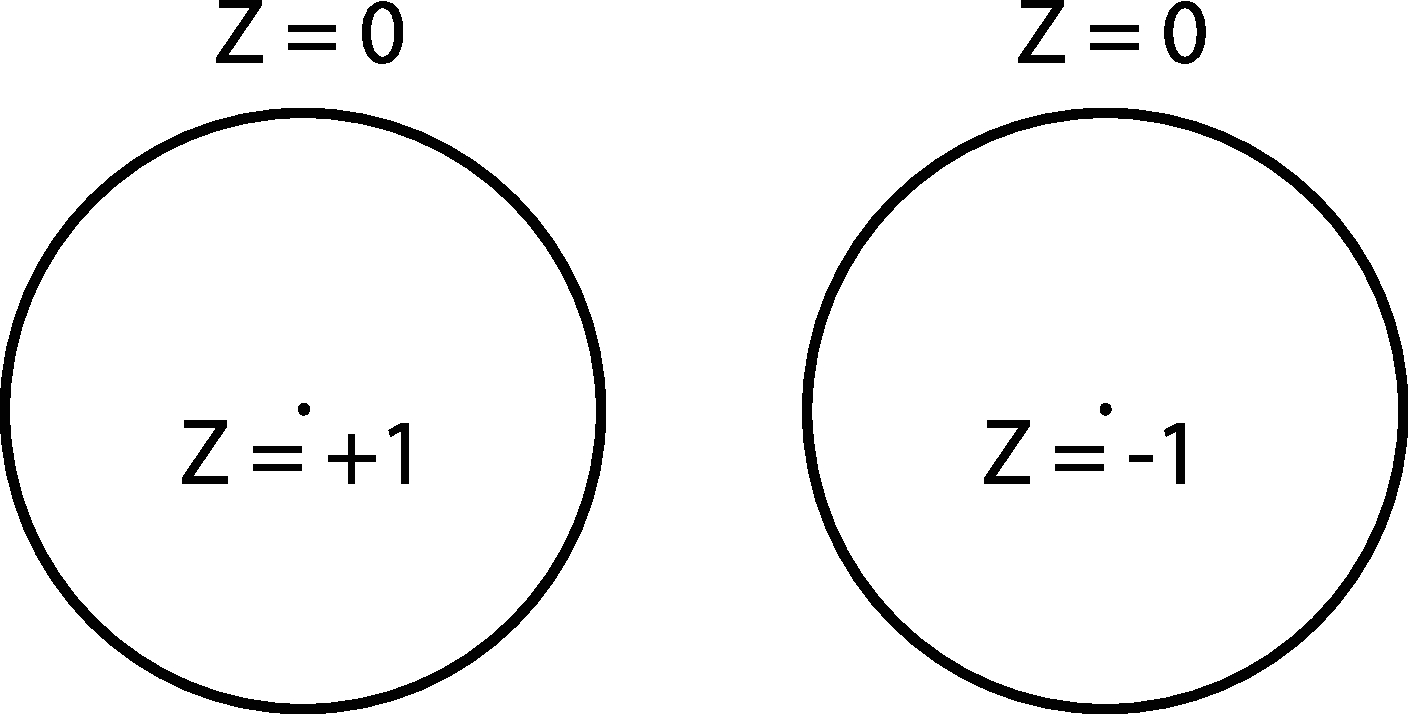
\includegraphics[scale=0.15]{src/images/chap26/14.jpg}
\end{figure}
\bigskip

The common part is the equator $z = 0$, i.e, $x^2 + y^2 = 1$ and we should think
of attaching the two disks there. With this hint we can now draw two balls,
the ~ ``northern" say $y^{\phantom{2}}_{L}  \geq 0$  \quad $x^2_R + y^2_R + x^2_L = 1 - y^2_L \leq 1$
\smallskip

{} \hspace{1.6cm} ``sourthern" $y^{\phantom{2}}_{L} \leq  0$ \quad  $x^2_R + y^2_R + x^2_L = 1 - y^2_L \leq 1$
\bigskip

\begin{figure}[H]
\centering
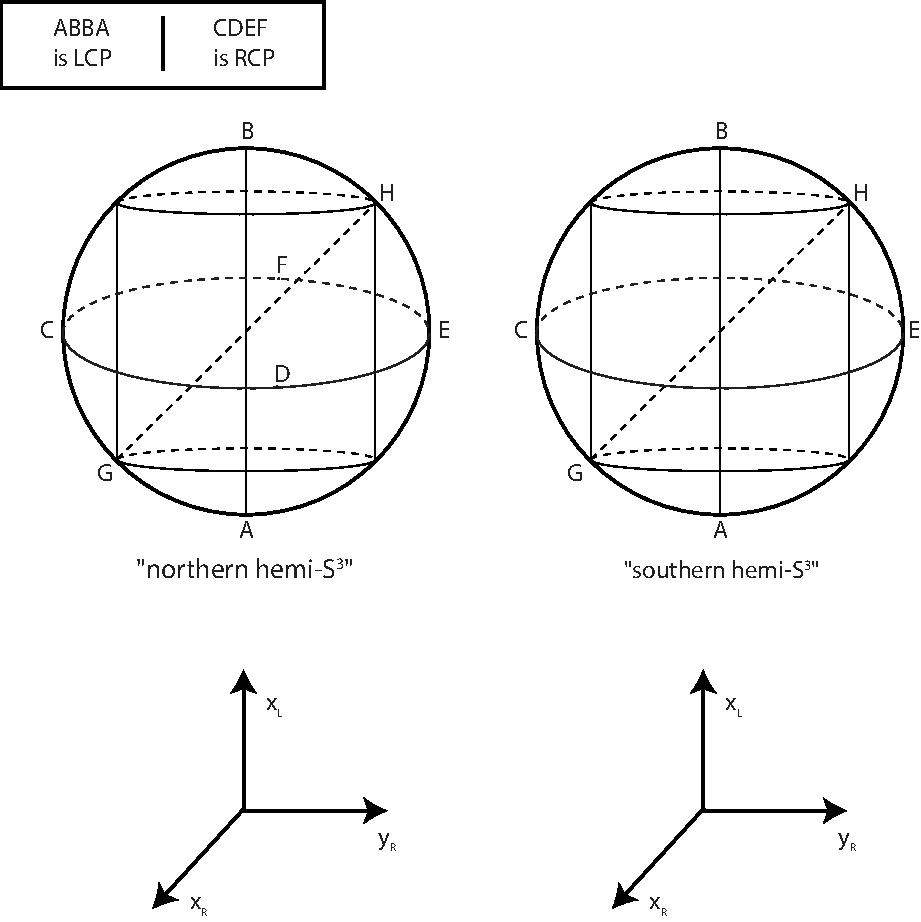
\includegraphics[scale=0.425]{src/images/chap26/15.jpg}
\end{figure}
\bigskip

Only one torus say $\theta  = \pi/4$ is shown and is one circle on this torus GHHG.
The remaining ircles on this torus can be obtained by rotation about the $x_L$ axis.
The family of linked non intersecting circles in $S^3$ is called the set of ``Clifford
parallels" after their discoverer. They
look different from each other because of our projection just as in geography,
but they are really similar in size and shape. The last piece of mathematics
we touch upon comes from $Hopf$. Since each circular orbit has fixed $\theta \phi$ and
lets phase vary, one is justified in saying we have a map from $S^3 (\theta, \xi_1, \xi_2)$ to
$S^2 (\theta, \phi)$ with $\phi = \xi_2 - \xi_1$. Going in the reverse direction, for each point ($\theta, \phi$) on
`the Poincare' sphere, we have a circle ($\theta, \xi_1,~ \xi_2$ with fixed $\xi_2 - \xi_1$). Generating, $S^3$ is the `total space', it is full of $S^1$ ``fibres" (one through each point) and the family of fibres itself is an $S^2$ (the Poincare' sphere) which is called the base.
A much more familiar example from high school is the $x - y$ plane of analytic
geometry which has $R^1$ fibres in which $y$ varies, labelled by another $R^1$ viz $x$.
\bigskip

\begin{figure}[H]
\centering
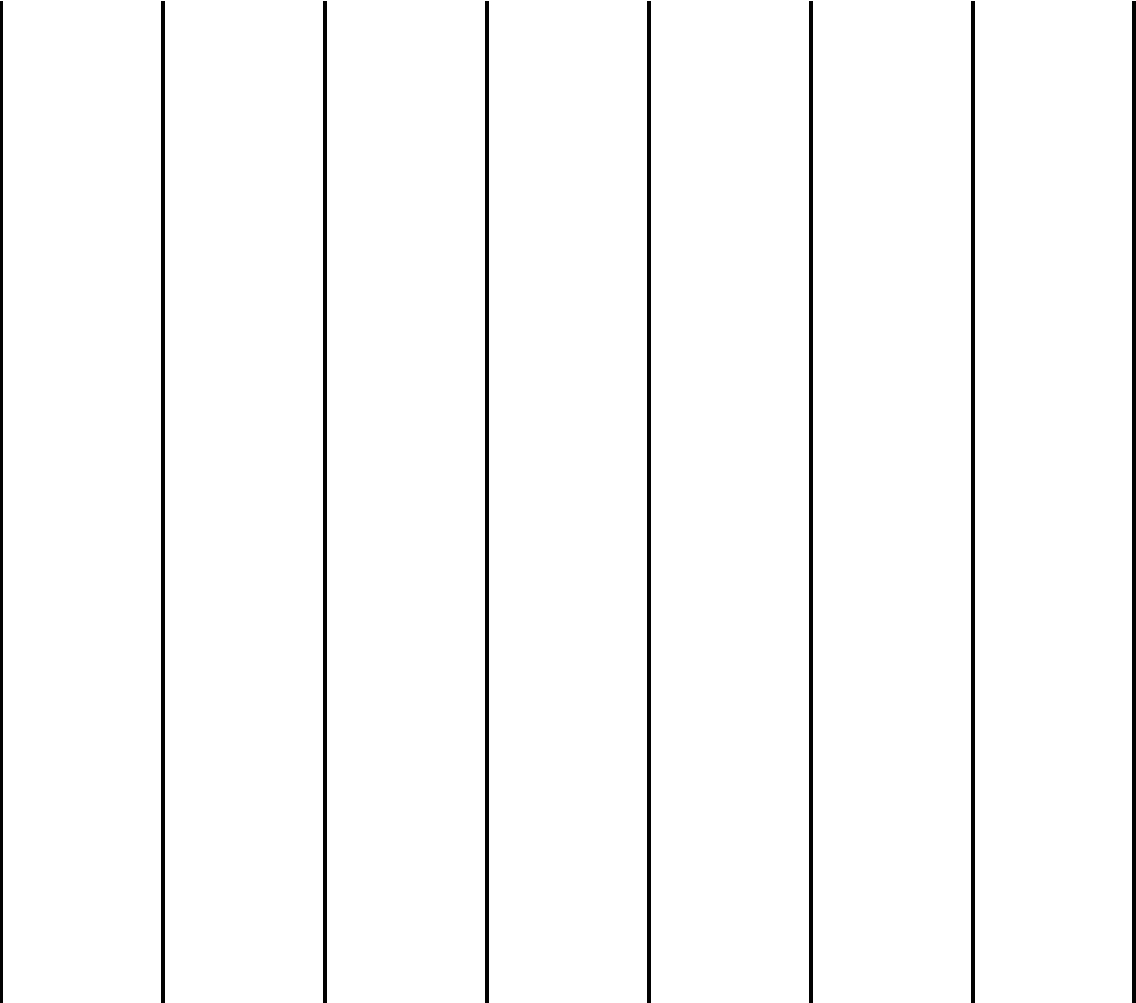
\includegraphics[scale=0.1]{src/images/chap26/16.jpg}
\end{figure}
\bigskip

In this case, we could equally have fibres labelled by $y$ along which $x$ - varies,
i.e, it is a cartesian product $R^1 \times R^1$. Just to show that not all the fibre bundles
are products, consider the M\"{o}bius surface sketched below.
\begin{figure}[H]
\centering
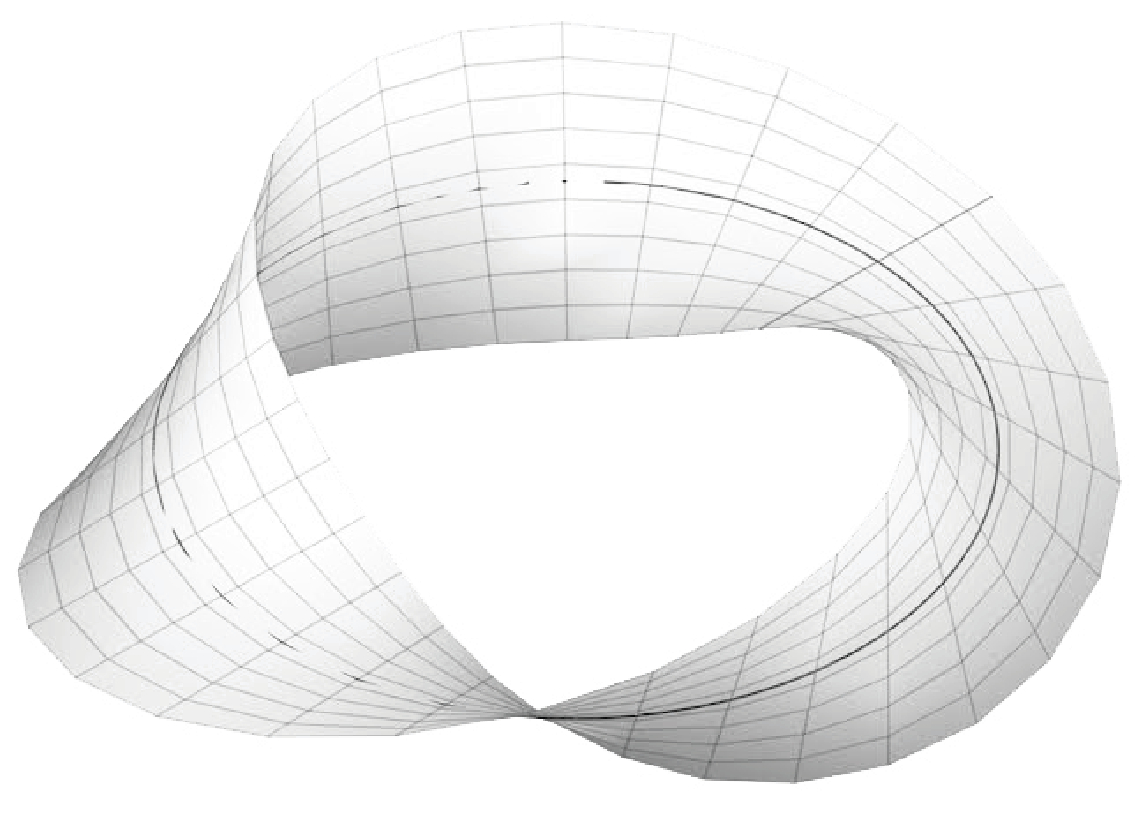
\includegraphics[scale=0.27]{src/images/chap26/17.jpg}
\end{figure}

It is a family of straight line segments whose centres lie on a circle (dashed
line). But if we try to introduce an $x$ co-ordinate on each segment foe each $\theta$,
say with the origin on the circle, we run into a discontinuity when we go around
once - positive $x$'s sit right next to negative ones - no surprise since the surface
was made by gluing after a $180^{\circ}$ twist. The moral is that a fibre bundle can
be `twisted' i.e, we can assign coordinates on each fibre, but we can't have smooth
coordinate surfaces which cut all the fibres, each only once.$^{\ast}$

Returnig to our three sphere $S^3$ which represents both polarisation and
phases we can now ask if there is a phase coordinate on each fibre (no problem,
its a circle) which is continuous for all of our polarisation states, i.e, for all $\theta \phi$
on `the Poincare' sphere? We loosely referred to $\xi_2 - \xi_1$ as twice the azimuth and
$\xi_1$ as overall phase, but $\xi_1$ fails at LCP, $\theta = \pi$. We could try and choose all the
states to be in phase with a given one - but this will fail at the antipodal point.
In graphic terms, the challenge is to place a dot (as a conventional origin of phase)
for all ellipses on `the Poincare' sphere in a continuous way - a failed attempt is
sketched below.
\bigskip

\begin{figure}[H]
\centering
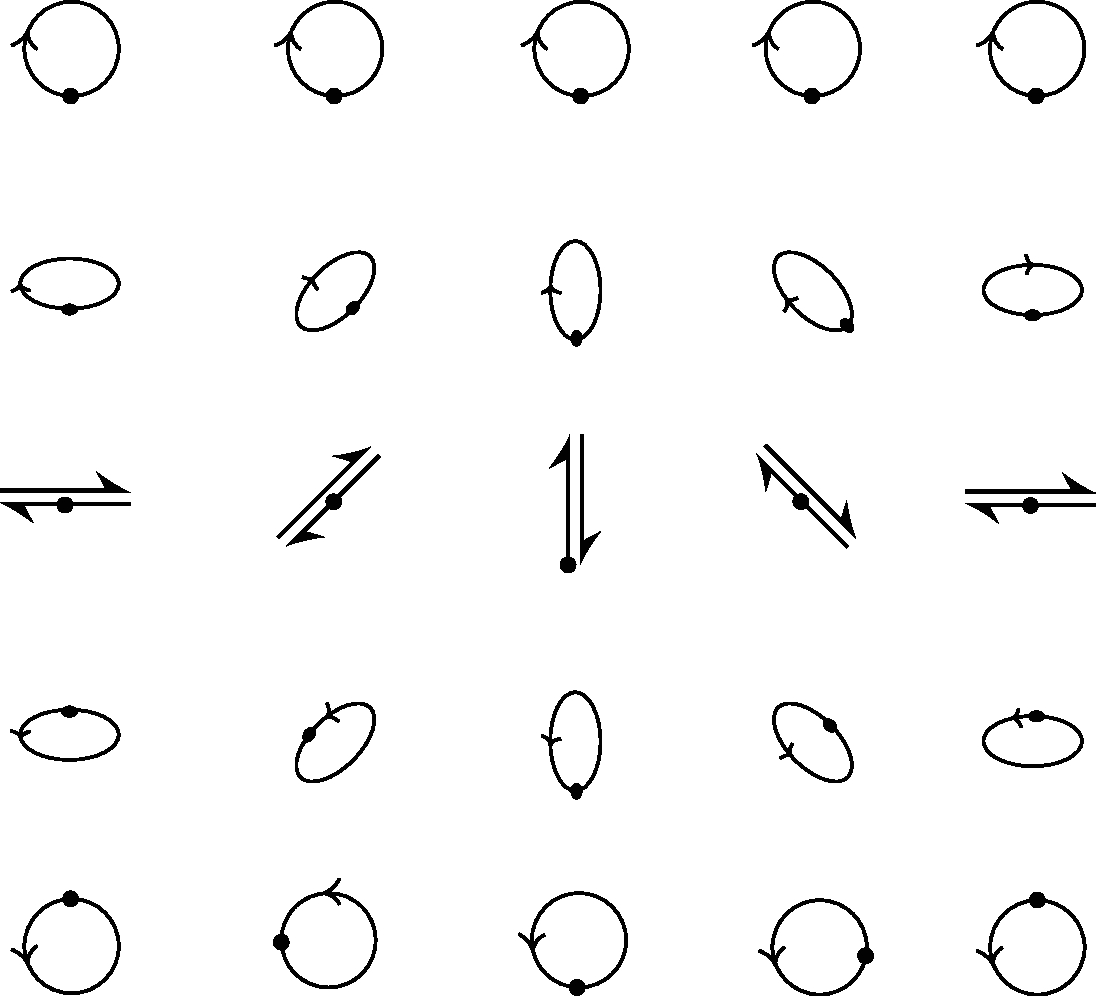
\includegraphics[scale=0.22]{src/images/chap26/18.jpg}
\end{figure}
\bigskip

In fact, all such attempts fail. Stated as geometrical fact, it implies that
in our diagram of $S^3$ on page --, it is immposible draw a smooth surface which
cuts each circle once and only once. An elementary proof (of a fact known
from the time $Hopf$ introduced his fibration) can be found in a paper I wrote in
\textit{Pramana} in March 1979 accessible by just typing `\textit{Impossibility of a continuous
phase convention for polarised light}' into a google window. This is a sure sign
that our total space is \underline{not} a product, $S^3$ is not $S^2 \times S^1$ (A topologist wouldn't
hesitate a second to say this - a closed loop along $S^1$ winding around it once
cannot be shrunk to a point, while all loops in $S^3$ can be).

In summary, the very simple sysytem of polarised light, or two harmonic
oscillators, leads us to a complex vector spaces, the projective version of them,
connections on these fibre bundles which are twisted in a basic way - all of which
are useful in unerstanding more advanced topics - quantum and otherwise. Good
return on investment!

Polarisation optics has one more geometric phase in store for us - which pre-dates \textit{Pancharatam} by thirty years, but again gained, prominence after Berry's work of 1984. It was well known from the beginnngs of geometrical optics that
when the refractive index varies with position, a ray of light describes a curved
path - the familiar mirage being an example. The figure shows how this is a consequence of
wavefronts slowing down where the refractive index is higher.
\bigskip

\begin{figure}[H]
\centering
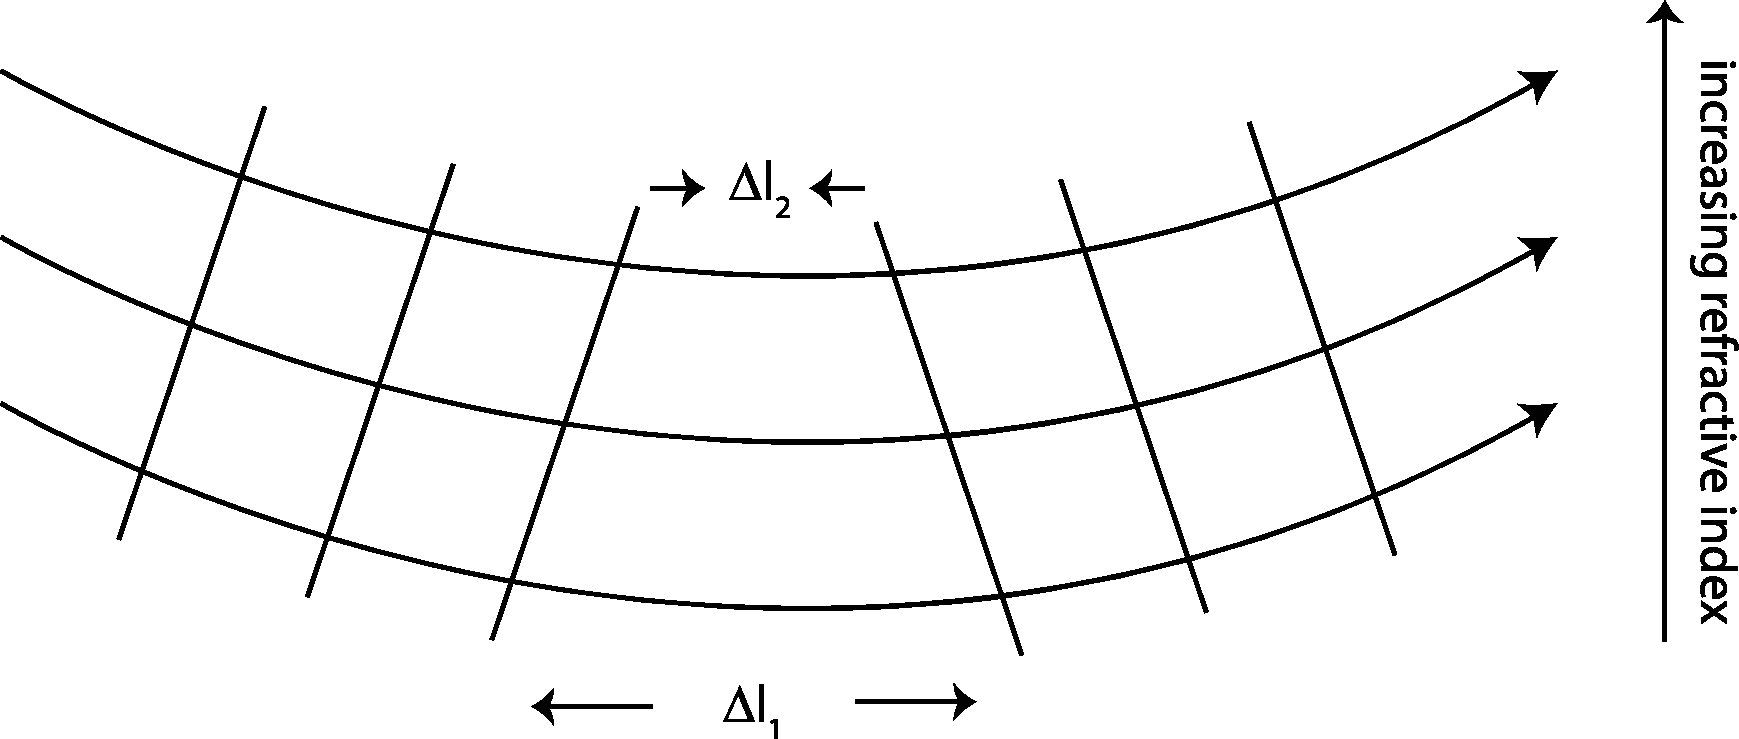
\includegraphics[scale=0.19]{src/images/chap26/19.jpg}
\end{figure}
\bigskip

Quantitatively the radius of curvature can eaisly\footnote{Just use the condition that the phase difference between two wavefronts is fixed, $n_1 \Delta \ell_1 = n_2 \Delta \ell_2$ in the sketch.} be calculated
$$
\frac{1}{R} = \frac{\nabla \perp n (x,y,z)}{n}
$$

The gradient is to be taken perpendicular to the ray, and its direction gives
the plane of curvature. So long as the ray traverses a plane curve, the behaviour
of the polarisation is fixed by symmetry. The component normal to the plane
stays constant. The component lying in the plane stays in the plane, but
turns in the same way as the ray so as to stay perpendicular to it. The question
of how polarisation varies becomes more subtle when the curve does not lie in
a plane which can happen as the vector $\nabla \perp n $ rotates in the plane perpendicular
to ray. The basic result is due to \textit{Bertolotti} (1926) and \textit{Rytor} (1937) but was
given a nice geometric form by \textit{Vladimirskii} (1941). This is illustrated for a curve in
the form of a helix.
\bigskip

\begin{figure}[H]
\centering
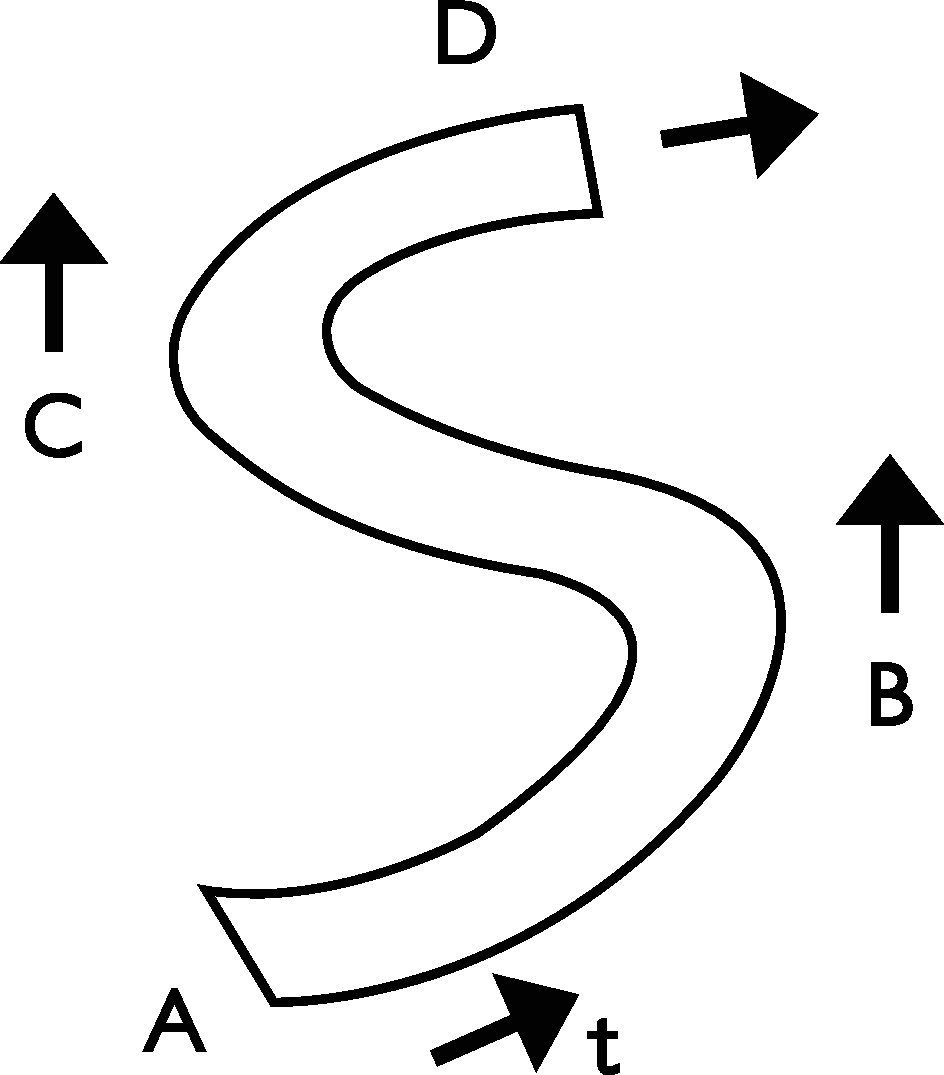
\includegraphics[scale=0.14]{src/images/chap26/20.jpg}
\end{figure}
\bigskip

Note that a unit tangent vector $\overrightarrow{t}$ describes a cone whic is completed after
one turn of the helix. This is shown in a separate ``direction space".
\bigskip

\begin{figure}[H]
\centering
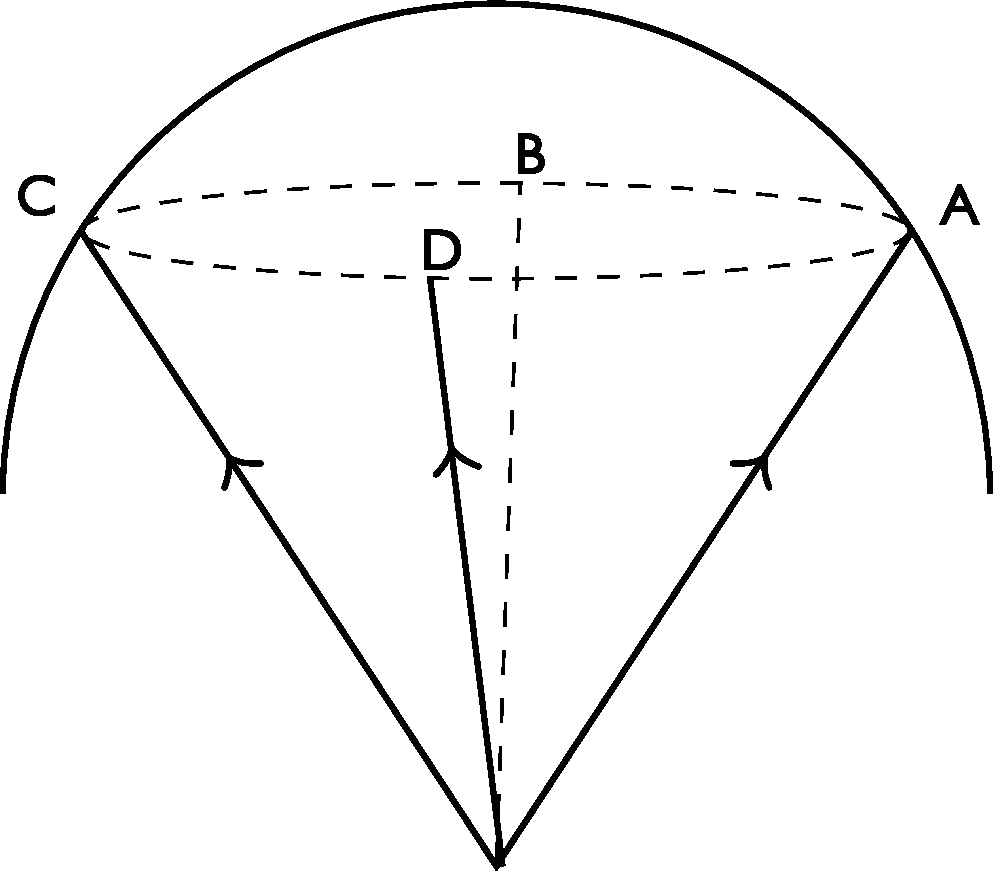
\includegraphics[scale=0.27]{src/images/chap26/21.jpg}
\end{figure}
\bigskip

Since the polarisation vector is always perpendicular $\hat{t}$, we can think of it as
living in a tangent plane to the sphere at the tip of $\hat{t}$. This situation was already
encountered in the geometry of curved surfaces (and higher dimensional spaces)
by none other than Bertolotti's guru, \textit{Tullio Levi Civita}. It is the intuitively
appealing notion of parallel displacement. Imagine a person sent on a long
journey on the earth with two instructions. ``Here is long pole, carry it so that
it remains parallel to the ground but do not otherwise turn it in any other way".
the result is shown in the sketch below.
\bigskip

\begin{figure}[H]
\centering
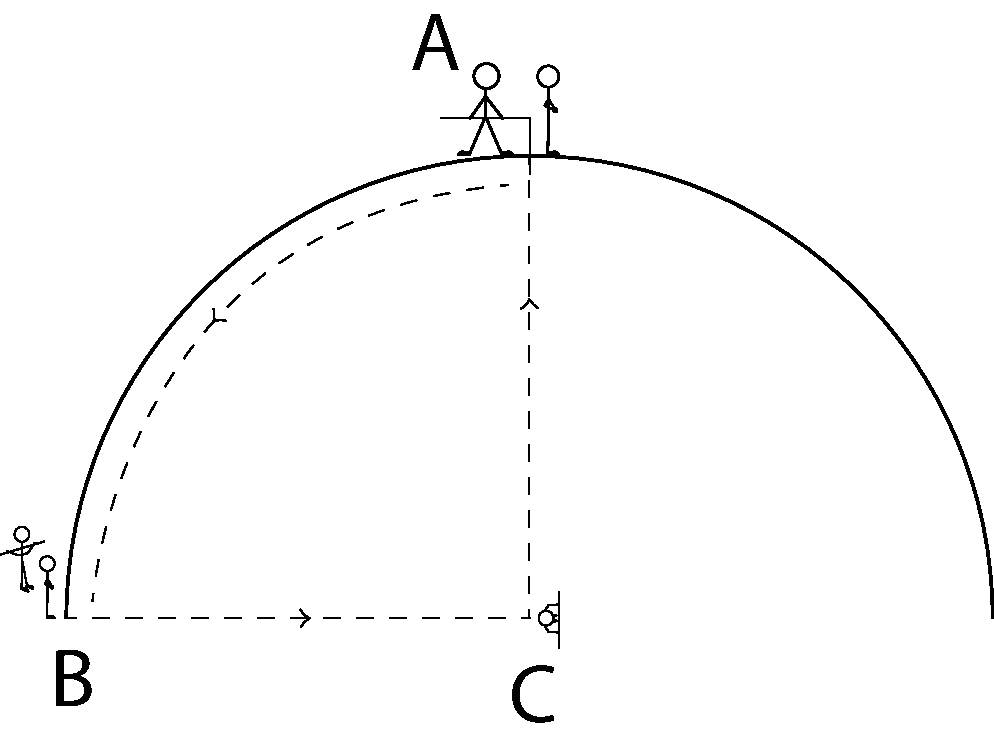
\includegraphics[scale=0.34]{src/images/chap26/22.jpg}
\end{figure}
\bigskip

At $B$ and $C$, the person turns but not the pole. Yet, on return to $A$, the pole
has turned from its original direction by $\frac{\pi}{2}$ (and in general the solid angle made
by $ABC$ at the centre). Vladimirskii's insight was that polarisation behaves
exactly in this way - Today this is demonstrated nicely using optical fibres.
But a rotation of linear polarisation is a phase difference (of twice that angle)
between $R$ and $L$! So now we have a geometric phase for change of direction.
Combining it with the \textit{Pancharatam} phase is an exercise for the reader!

My first overlap with Prof G. Ramachandran was attending a seminar he gave in the
Department of physics of the Indian Institute of Science, which was unusually, on particle
physics. Later, from my association with Pramana, I became familiar with the school he had
established at Mysore working broadly on `spin physics'. During later visits to the
department and the Academic Staff college, I got to know his students many of whom are
themselves dedicated teachers and researchers and contributors to this volume. This kind
of impact and legacy is quite rare in the university system and I am happy to contribute this
article which commemorates such an outstanding academic. Appropriately, the lectures on
which this article is based were delivered in physics department of the University of
Mysore, so this article also expresses my gratitude for the welcome I have always received in
that community.
\vskip 1cm


\centerline{
\includegraphics[scale=0.9]{authorsphotos/Prof_Rajaram_Nityananda.jpg}} 
\bigskip

\noindent
\textbf{Dr.\ R. Nityananda} carried out his research at NAL, Bangalore, and obtained the Ph.D. degree from Bangalore University in 1977. He joined Raman Research Institute, Bangalore, in 1975 and worked there till the year 2000.  He was the Centre Director, NCRA-TIFR, Pune, during 2000 to 2010. Currently he is a Senior Professor at Azim Premji University, Bengaluru.
